\documentclass[crop,tikz]{standalone}
\usetikzlibrary{backgrounds}
\colorlet{blue}{cyan}
\tikzset{
  inverted/.style = {
    every path/.style = {draw=white,text=white},
    background rectangle/.style={fill},
    show background rectangle
  }
}

\tikzset{>=latex}
\colorlet{green}{green}
\newcommand{\place}{\vec{r}}

\begin{document}
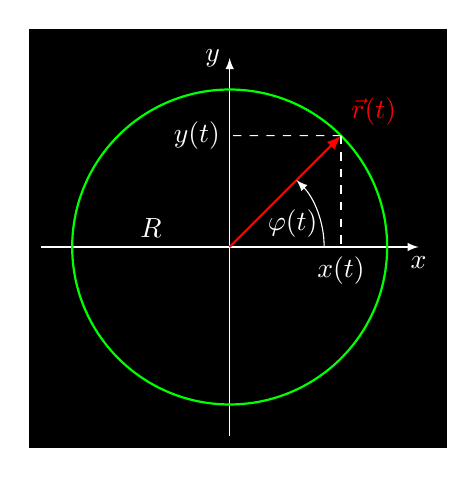
\begin{tikzpicture}[inverted,scale=2]
    \draw[->] (-1.2,0) -- (1.2,0) node[below] {$x$};
    \draw[->] (0,-1.2) -- (0,1.2) node[left] {$y$};
    \draw[green, thick] (0,0) circle (1);
    \draw[->,thick,red] (0,0) -- (45:1) node[right,anchor=south west]{$\place(t)$};
    \draw[->] (0.6,0) arc (0:45:0.6);
    \draw (0.4,0) node[above] {$\varphi(t)$};
    \draw (-0.5,0) node[above] {$R$};
    \draw[dashed] (0.707,0.707) -- (0.707,0) node[below] {$x(t)$};
    \draw[dashed] (45:1) -- (0,0.707) node[left] {$y(t)$};
\end{tikzpicture}
\end{document}
